% \section{Atividades}
%
% Neste módulo, foram realizadas atividades práticas voltadas ao monitoramento,
% auditoria e análise de eventos em ambientes Linux e Windows Server 2022, com
% foco na inspeção de logs, sincronização de tempo em rede e captura de tráfego.
%
% As tarefas contemplaram a exploração de registros do sistema no Windows Server
% 2022, a habilitação do protocolo NTP utilizando servidor externo, a análise de
% logs no Kali Linux por linha de comando e interface gráfica, além da captura e
% inspeção de pacotes com \textit{Wireshark} e \textit{tcpdump} em conexões TLS.
%
% Cada atividade apresenta abaixo o respectivo print solicitado, acompanhado de
% descrição explicativa conforme exigido nas orientações do módulo.
%
% \newpage
%
\question[Atividade 12.1]{Explorando os Logs no Windows Server 2022}

\begin{figure}[H]
\centering
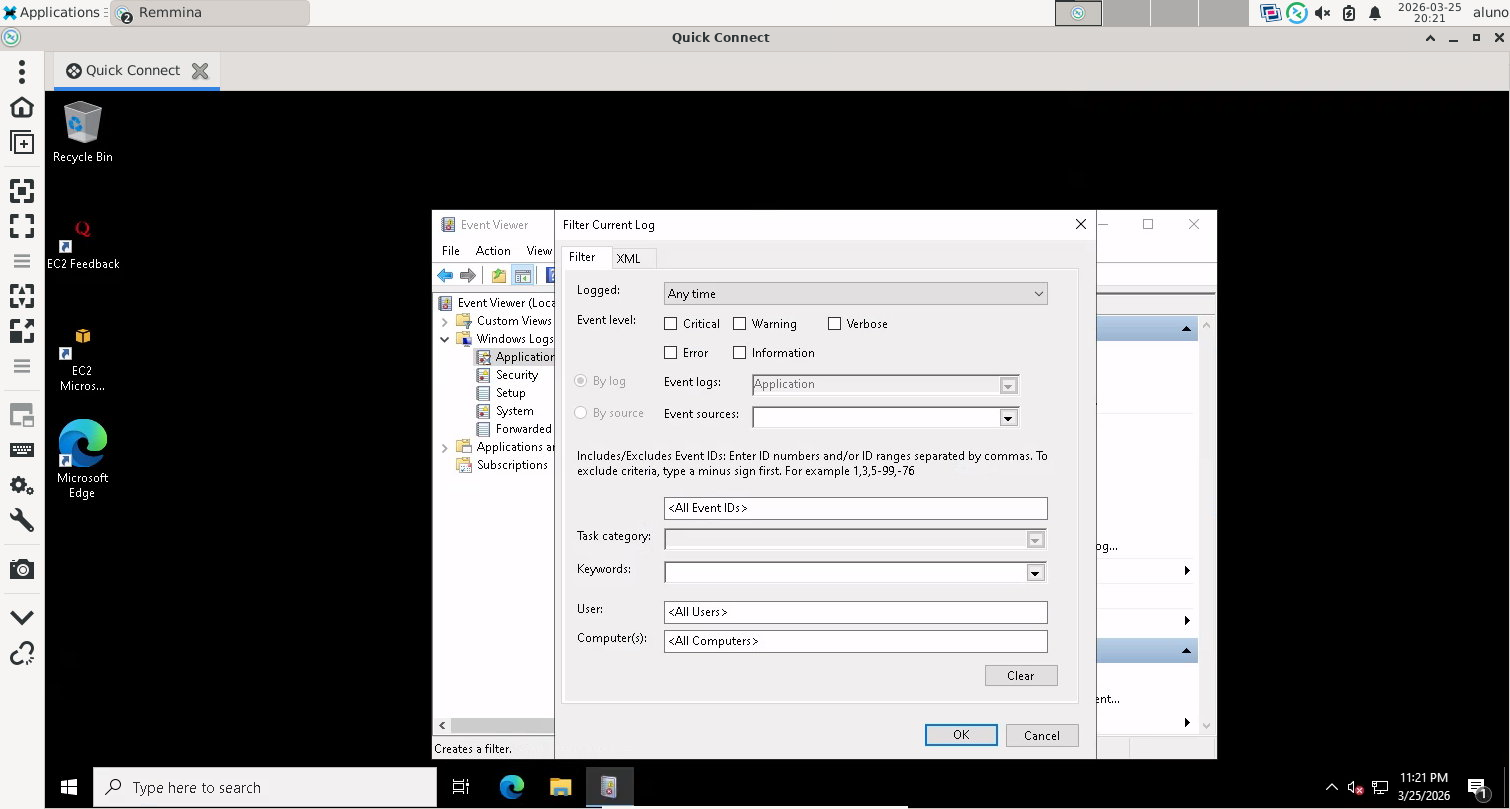
\includegraphics[width=0.99\textwidth]{./fig/fig12.1.png}
\caption{Janela Filter Current Log no Event Viewer do Windows Server 2022}
\label{fig:fig12.1}
\end{figure}

\newpage

\question[Atividade 12.2]{Habilitando o NTP no Windows Server 2022}

\begin{figure}[H]
\centering
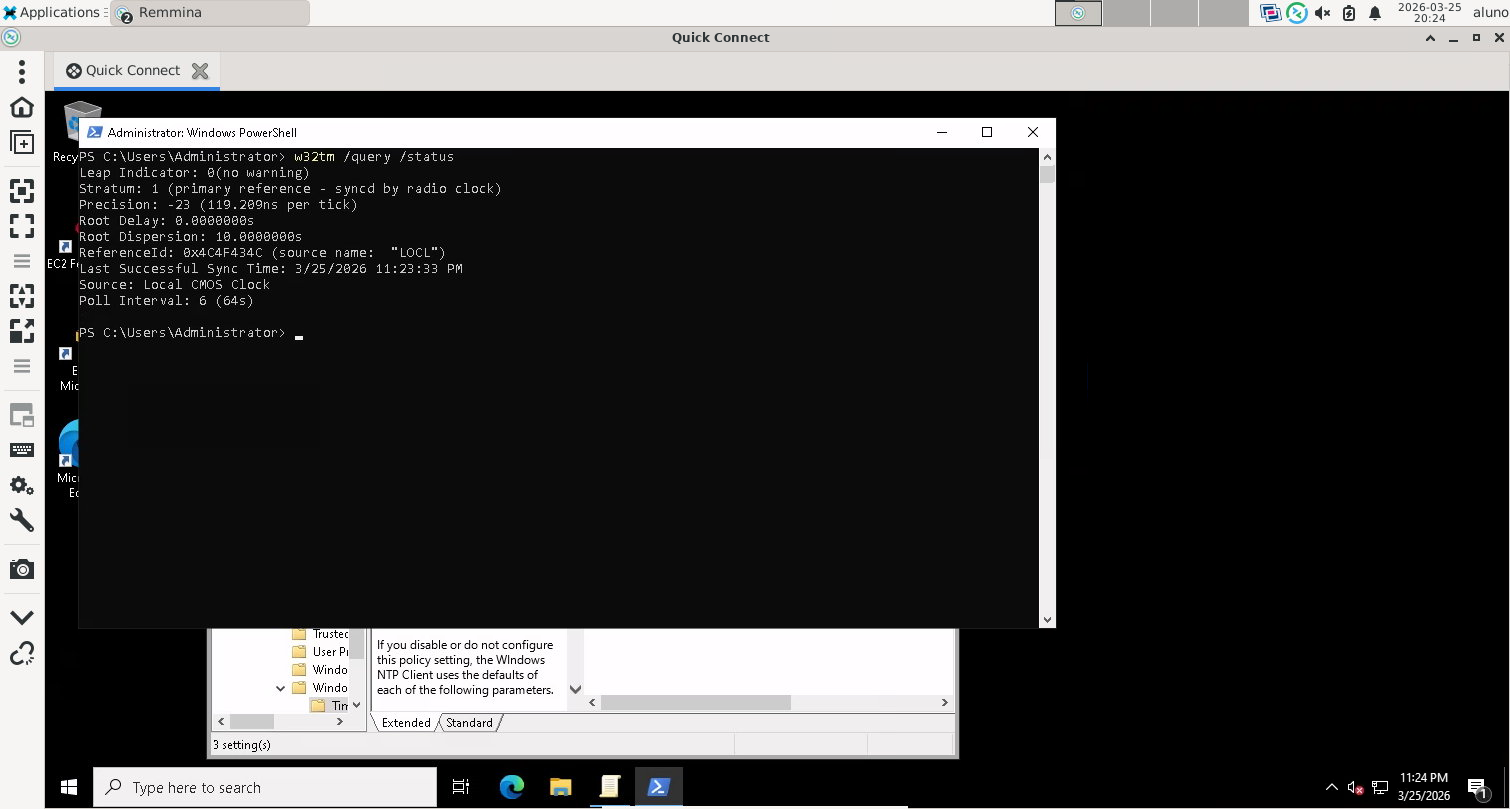
\includegraphics[width=0.99\textwidth]{./fig/fig12.2.png}
\caption{Resultado do comando w32tm /query /status após configuração do NTP}
\label{fig:fig12.2}
\end{figure}

\newpage

\question[Atividade 12.3]{Explorando os Logs no Kali Linux}

\begin{figure}[H]
\centering
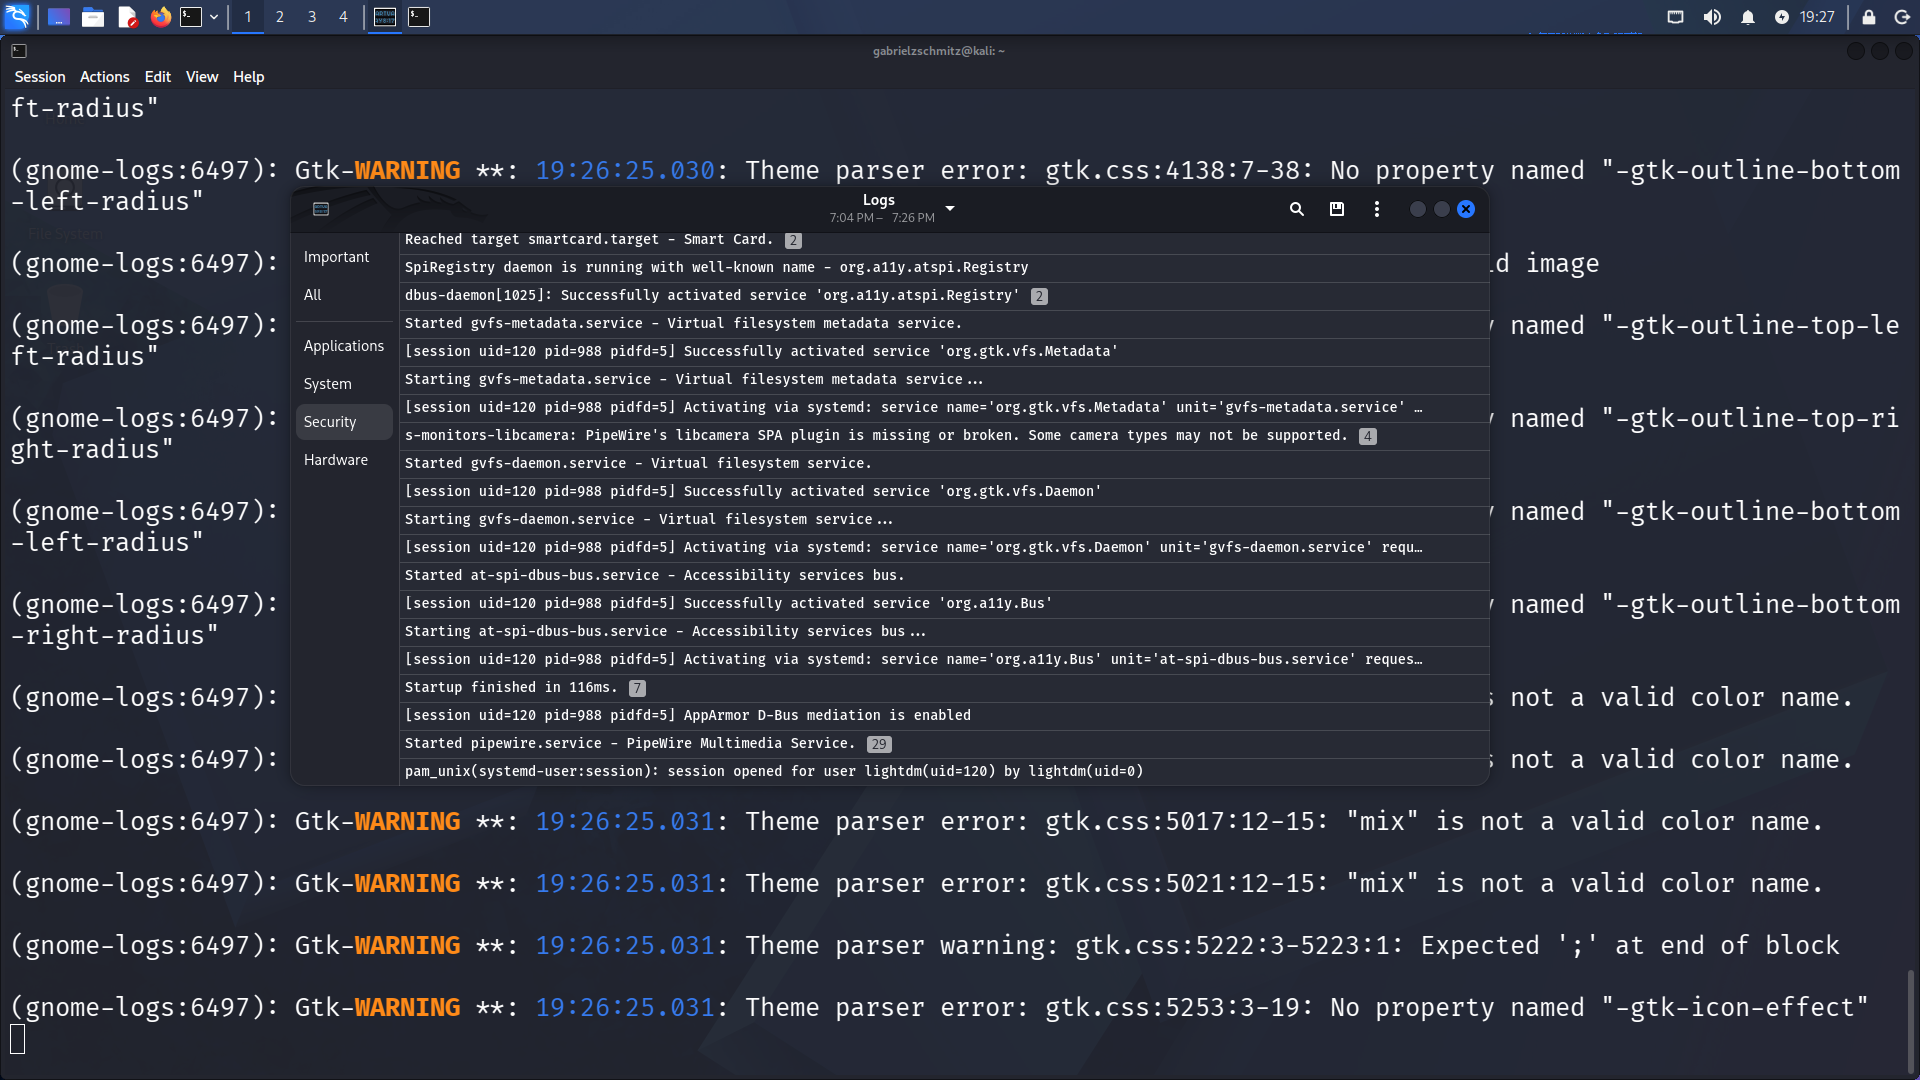
\includegraphics[width=0.99\textwidth]{./fig/fig12.3.png}
\caption{Visualização de logs de segurança no utilitário gnome-logs do Kali Linux}
\label{fig:fig12.3}
\end{figure}

\newpage

\question[Atividade 12.4]{Capturando pacotes com Wireshark no Kali Linux}

\begin{figure}[H]
\centering
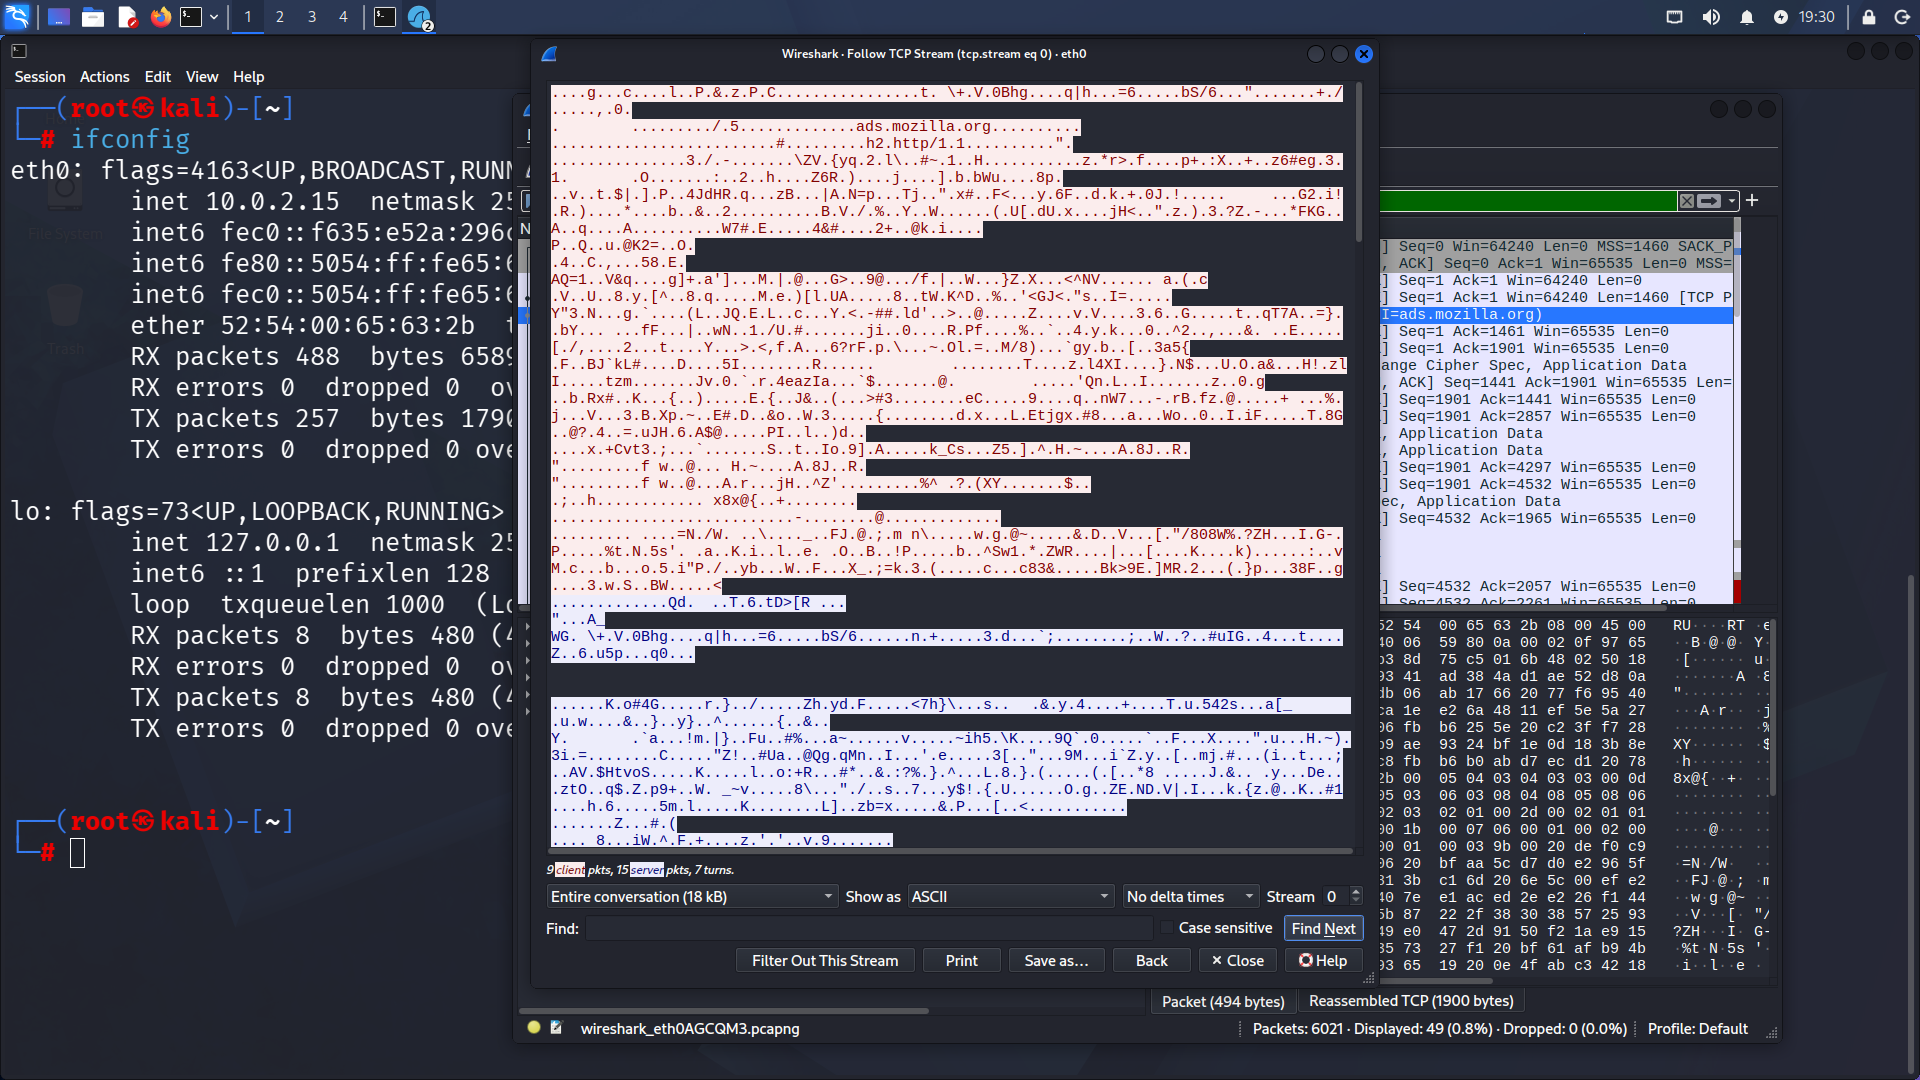
\includegraphics[width=0.99\textwidth]{./fig/fig12.4.png}
\caption{Fluxo TCP criptografado observado no Wireshark durante análise HTTPS}
\label{fig:fig12.4}
\end{figure}

\newpage

\question[Atividade 12.5]{Analisando pacotes TLS com tcpdump e Wireshark}

\begin{figure}[H]
\centering
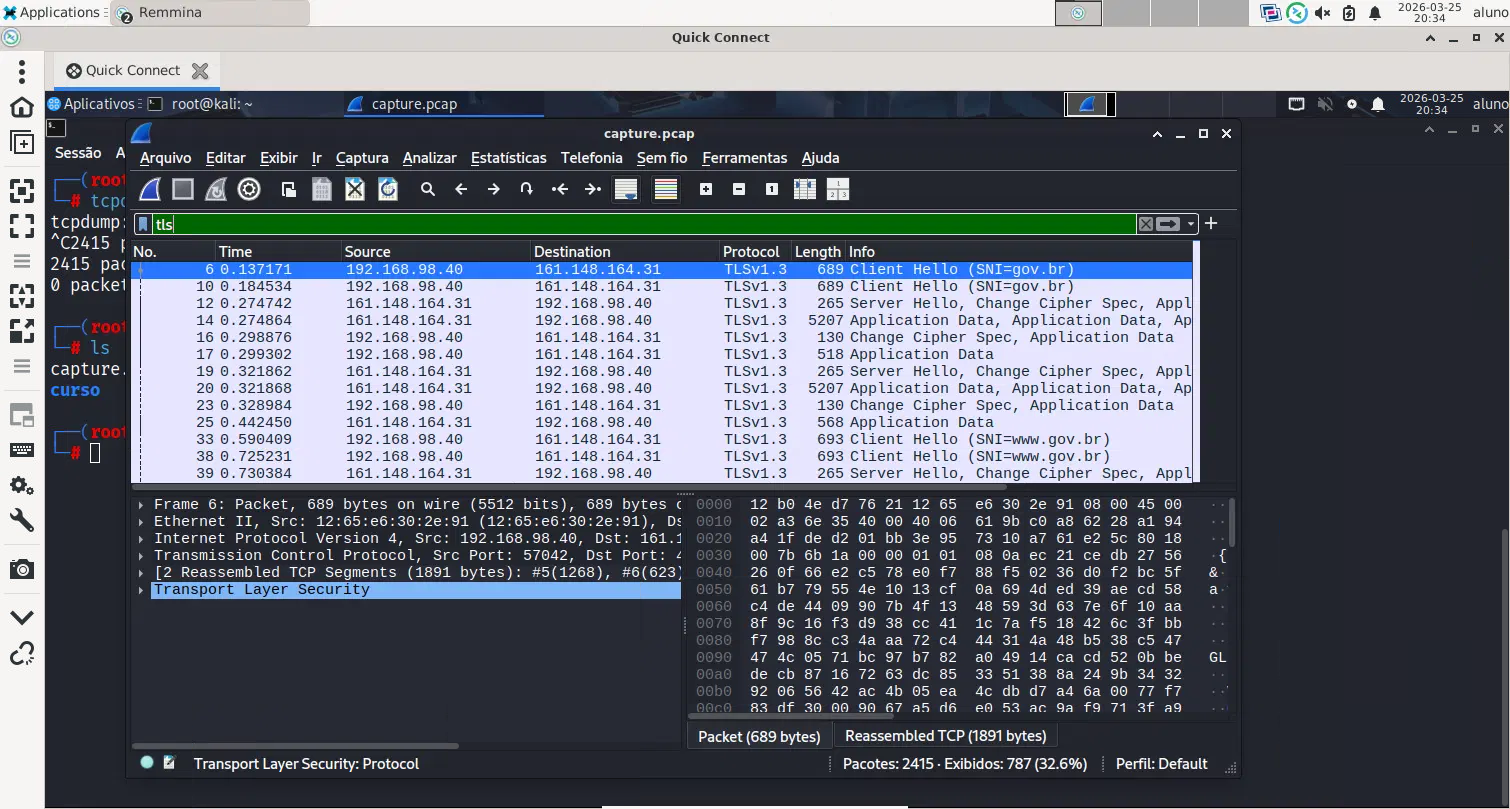
\includegraphics[width=0.99\textwidth]{./fig/fig12.5.png}
\caption{Pacotes TLS filtrados no Wireshark após captura com tcpdump}
\label{fig:fig12.5}
\end{figure}
